% L14a lecture companion. Notebook hashes and coverage are recorded in README.md.
% Style files and Cornell seal are copied unchanged from the L13a deck (identical
% to L13c, L12c, L12a, L10c, L10a, L9c, and L9a, which match the approved L6a
% deck). The two figures are the light TikZ PDFs in ../figs (Fig-Eigenvectors
% and Fig-PhasePortraits).
%
% Notation follows the lecture: the state x(t) in R^n (n states), the input
% u(t) in R^d (d inputs), the state matrix A in R^{n x n}, the input matrix B in
% R^{n x d}, the initial state x_0, the n x n identity I, the matrix exponential
% e^{At}, eigenvectors v in C^n and eigenvalues lambda in C, the eigenvector
% matrix V and the diagonal eigenvalue matrix Lambda, the coefficients c = V^{-1}
% x_0, lambda = alpha + i beta, the trace tau and the determinant det(A), the
% grid t_k = k Delta t, the held input u_k, the discrete matrices Abar and Bbar,
% the discrete eigenvalue lambdabar, the nonlinear model x' = f(x,u) with
% entries f_i, the operating point (x_op, u_op), the deviations Delta x and
% Delta u (capital Delta, a difference like Delta t), the Jacobian entries a_ij
% and b_ij, the constant f_op, and the steady state (x*, u*).
\documentclass[aspectratio=169,11pt]{beamer}
\usepackage{vnslides}
\renewcommand{\vnlecturecode}{L14a}
\newcommand{\lecturelink}{https://github.com/varnerlab/CHEME-5800-CourseRepository-Fall-2026/blob/main/weeks/week-14/L14a/CHEME-5800-L14a-Lecture-LinearStateSpaceModels-Fall-2026.ipynb}
\newcommand{\examplelink}{https://github.com/varnerlab/CHEME-5800-CourseRepository-Fall-2026/blob/main/weeks/week-14/L14a/CHEME-5800-L14a-Example-GeneCircuits-Fall-2026.ipynb}
\newcommand{\eigenlink}{https://github.com/varnerlab/CHEME-5800-CourseRepository-Fall-2026/blob/main/weeks/week-14/L14a/CHEME-5800-L14a-Advanced-ComputingEigenvalues-Fall-2026.ipynb}
\newcommand{\bilinearlink}{https://github.com/varnerlab/CHEME-5800-CourseRepository-Fall-2026/blob/main/weeks/week-14/L14a/CHEME-5800-L14a-Advanced-Derivation-BilinearStability-Fall-2026.ipynb}
\newcommand{\lecturesource}[1]{\note{[Sources]\par
  \href{\lecturelink}{L14a lecture: Linear State Space Models and Stability.}\par
  #1\par[/Sources]}}
\newcommand{\op}{\text{op}}

\title{\texorpdfstring{{\vnheavy L14a}: Linear State Space Models and Stability}{L14a: Linear State Space Models and Stability}}
\subtitle{\texorpdfstring{Eigenvalues, discretization, and linearization\\[3pt]CHEME 5800 Cornell University}{Eigenvalues, discretization, and linearization; CHEME 5800 Cornell University}}
\author{Copyright Jeffrey Varner 2026. All Rights Reserved}

\begin{document}
\special{pdf:minorversion 7}
\vntitlepage

\begin{frame}{Objectives for Today}
  When we push a system away from a steady state, does it come back?

  \vspace{0.4em}
  {\large\textbf{\ink{Today's concepts}}}
  \vspace{0.2em}
  \begin{itemize}\setlength{\itemsep}{0.4em}
    \item \hilite{Solve the open-loop model and read its stability}: without an
      input, the solution is a sum of modes, one for each eigenvalue of the
      state matrix. The real part of each eigenvalue decides whether its mode
      grows or decays.
    \item \hilite{Solve the forced model one time step at a time}: with an
      input, the solution contains an integral of the input over time. We
      derive two discretizations, the bilinear and the zero-order hold.
    \item \hilite{Linearize a nonlinear model about an operating point}: a
      first-order Taylor expansion gives a linear model whose matrices are
      Jacobians. Its eigenvalues give the stability of a steady state.
  \end{itemize}
  \slidenote{Lecture:}{\href{\lecturelink}{Linear State Space Models and Stability}}
  \lecturesource{Introduction and three Learning Objectives.}
\end{frame}

\begin{frame}{Lecture and Example}
  \textbf{\ink{Lecture:}}
  \href{\lecturelink}{Linear State Space Models and Stability}

  In this lecture, we solve linear time-invariant state space models, in which
  the state changes at a rate set by the current state and an input. We read the
  stability of a model from the eigenvalues of its state matrix. Then we
  linearize a nonlinear model about an operating point.

  \vspace{1.1em}
  \textbf{\ink{Example:}}
  \href{\examplelink}{Linearize a gene circuit}

  In this example, we build the model of a gene circuit from its config file
  and solve it with an ODE solver. We linearize the model about its steady
  state, and solve the linear model with the bilinear or the zero-order hold
  discretization.
  \lecturesource{Introduction and the Examples section.}
\end{frame}

\begin{frame}{Linear State Space Models}
  A \hilite{linear time-invariant (LTI) state space model} describes how a
  vector of states changes over time in response to an input:
  \[
    \boxed{\dot{\mathbf{x}}(t)=\mathbf{A}\mathbf{x}(t)+\mathbf{B}\mathbf{u}(t),\qquad \mathbf{x}(0)=\mathbf{x}_{0}}
  \]
  \vspace{-0.4em}
  \begin{itemize}\setlength{\itemsep}{0.35em}
    \item $\mathbf{x}(t)\in\mathbb{R}^{n}$ is the vector of $n$ states, such as
      the concentrations in a reactor. The time derivative of the state is
      $\dot{\mathbf{x}}$, and $\mathbf{x}_{0}\in\mathbb{R}^{n}$ is the initial
      state.
    \item $\mathbf{u}(t)\in\mathbb{R}^{d}$ is the vector of $d$ inputs, what we
      set from outside, such as a feed rate.
    \item $\mathbf{A}\in\mathbb{R}^{n\times n}$ is the \hilite{state matrix},
      and $\mathbf{B}\in\mathbb{R}^{n\times d}$ is the \hilite{input matrix}.
  \end{itemize}

  \vspace{0.4em}
  The model is \hilite{time-invariant} because $\mathbf{A}$ and $\mathbf{B}$ do
  not depend on $t$.
  \lecturesource{Linear State Space Models: the opening sentence, the continuous-time LTI box, and the paragraph on the state and the input.}
\end{frame}

\begin{frame}{The Open-Loop Solution}
  In the \hilite{open-loop} case, the input is zero, $\mathbf{u}=\mathbf{0}$,
  and the model reduces to $\dot{\mathbf{x}}=\mathbf{A}\mathbf{x}$. Its solution
  is given by the \hilite{matrix exponential}:
  \[
    \mathbf{x}(t)=e^{\mathbf{A}t}\mathbf{x}_{0},\qquad
    e^{\mathbf{A}t}=\mathbf{I}+\mathbf{A}t+\frac{(\mathbf{A}t)^{2}}{2!}+\frac{(\mathbf{A}t)^{3}}{3!}+\dots
  \]
  where $\mathbf{I}$ is the $n\times n$ identity matrix.

  \vspace{0.5em}
  \begin{itemize}\setlength{\itemsep}{0.5em}
    \item Differentiating the series term by term gives
      $\frac{d}{dt}e^{\mathbf{A}t}=\mathbf{A}e^{\mathbf{A}t}$. This solution
      satisfies the model.
    \item At $t=0$, the series gives $e^{\mathbf{0}}=\mathbf{I}$ and the
      initial state $\mathbf{x}_{0}$.
  \end{itemize}
  \lecturesource{Linear State Space Models: the open-loop case, the matrix exponential, and the two checks.}
\end{frame}

\begin{frame}{Eigenvectors and the Eigendecomposition}
  An \hilite{eigenvector} $\mathbf{v}$ of $\mathbf{A}$ is a nonzero vector that
  $\mathbf{A}$ only stretches, and the stretch factor $\lambda$ is its
  \hilite{eigenvalue}:
  \[
    \mathbf{A}\mathbf{v}=\lambda\mathbf{v},\qquad \mathbf{v}\in\mathbb{C}^{n},\quad \lambda\in\mathbb{C}
  \]
  Both can be complex, where $\mathbb{C}$ is the set of complex numbers.

  \vspace{0.5em}
  When $\mathbf{A}$ has $n$ linearly independent eigenvectors, its
  \hilite{eigendecomposition} and every power $\mathbf{A}^{k}$ are:
  \[
    \mathbf{A}=\mathbf{V}\boldsymbol{\Lambda}\mathbf{V}^{-1},\qquad
    \mathbf{A}^{k}=\mathbf{V}\boldsymbol{\Lambda}^{k}\mathbf{V}^{-1}
  \]
  where the columns of the $n\times n$ matrix $\mathbf{V}$ are the eigenvectors
  $\mathbf{v}_{1},\dots,\mathbf{v}_{n}$, and the $n\times n$ diagonal matrix
  $\boldsymbol{\Lambda}$ holds the eigenvalues $\lambda_{1},\dots,\lambda_{n}$.
  \slidenote{Advanced:}{\href{\eigenlink}{Computing eigenvalues with power iteration and QR iteration}}
  \lecturesource{Modes and the Eigendecomposition: the eigenvector definition and the eigendecomposition. Examples section: the advanced eigenvalue notebook.}
\end{frame}

\begin{frame}{Modes}
  Every power keeps the form $\mathbf{A}^{k}=\mathbf{V}\boldsymbol{\Lambda}^{k}\mathbf{V}^{-1}$,
  because each inner $\mathbf{V}^{-1}\mathbf{V}=\mathbf{I}$ cancels. We substitute
  these powers and $\mathbf{I}=\mathbf{V}\mathbf{V}^{-1}$ into the series:
  \begin{align*}
    e^{\mathbf{A}t} &= \mathbf{V}\left(\mathbf{I}+\boldsymbol{\Lambda}t+\tfrac{(\boldsymbol{\Lambda}t)^{2}}{2!}+\dots\right)\mathbf{V}^{-1}
      =\mathbf{V}e^{\boldsymbol{\Lambda}t}\mathbf{V}^{-1}\\
    \mathbf{x}(t) &= \mathbf{V}e^{\boldsymbol{\Lambda}t}\mathbf{V}^{-1}\mathbf{x}_{0}
      =c_{1}e^{\lambda_{1}t}\mathbf{v}_{1}+\dots+c_{n}e^{\lambda_{n}t}\mathbf{v}_{n}
  \end{align*}
  where $e^{\boldsymbol{\Lambda}t}=\operatorname{diag}(e^{\lambda_{1}t},\dots,e^{\lambda_{n}t})$,
  because each power of $\boldsymbol{\Lambda}$ is diagonal.

  \vspace{0.5em}
  \begin{itemize}\setlength{\itemsep}{0.5em}
    \item The coefficients $c_{1},\dots,c_{n}$, the entries of
      $\mathbf{c}=\mathbf{V}^{-1}\mathbf{x}_{0}$, express the initial state in
      the eigenvector basis.
    \item Each term $c_{i}e^{\lambda_{i}t}\mathbf{v}_{i}$ is a \hilite{mode} of
      the model. A mode keeps the direction of its eigenvector, and its size
      changes as $e^{\lambda_{i}t}$.
  \end{itemize}
  \lecturesource{Modes and the Eigendecomposition: the mode expansion and the paragraph after it.}
\end{frame}

\begin{frame}{Eigenvectors and Modes}
  \centering
  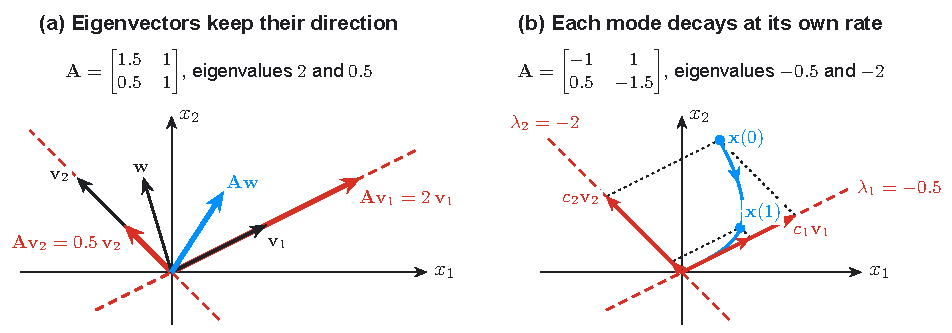
\includegraphics[width=\textwidth,height=0.60\paperheight,keepaspectratio]{assets/Fig-Eigenvectors.pdf}

  \vspace{0.4em}
  \raggedright
  (a) $\mathbf{A}$ stretches each eigenvector along its own line, while a
  general vector $\mathbf{w}$ changes direction. (b) By $t=1$, the fast mode
  has shrunk by $e^{-2}$ and the slow mode by $e^{-0.5}$, which bends the
  solution toward $\mathbf{v}_{1}$.
  \lecturesource{Modes and the Eigendecomposition: the eigenvectors and modes figure and its caption.
    Figure: ../figs/Fig-Eigenvectors/Fig-Eigenvectors.pdf (light TikZ build).}
\end{frame}

\begin{frame}{Growth, Decay, and Oscillation}
  Write a complex eigenvalue as $\lambda=\alpha+i\beta$, with real part
  $\alpha$ and imaginary part $\beta$. Euler's formula then gives:
  \[
    e^{\lambda t}=\underbrace{e^{\alpha t}}_{\updownarrow}\,\cdot\,\overbrace{\left(\cos\beta t+i\sin\beta t\right)}^{\text{oscillation}}
  \]
  \vspace{-0.3em}
  \begin{itemize}\setlength{\itemsep}{0.5em}
    \item The real part $\alpha$ sets the growth or decay of the mode, and the
      imaginary part $\beta$ sets its oscillation.
    \item A real eigenvalue has $\beta=0$, and its mode does not oscillate.
    \item Complex eigenvalues of a real matrix come in conjugate pairs,
      $\alpha\pm i\beta$. For a real initial state, the pair gives a real
      oscillation.
  \end{itemize}
  \lecturesource{Stability from the Eigenvalues: the complex eigenvalue, Euler's formula, and the paragraph after it.}
\end{frame}

\begin{frame}{Stability of the Open-Loop Model}
  A \hilite{steady state} is a state where $\dot{\mathbf{x}}=\mathbf{0}$, such
  as $\mathbf{x}=\mathbf{0}$.

  \vspace{0.5em}
  \begin{columns}[T,onlytextwidth]
    \begin{column}{0.47\textwidth}
      The steady state $\mathbf{x}=\mathbf{0}$ is:
      \begin{itemize}\setlength{\itemsep}{0.4em}
        \item \hilite{stable} when every eigenvalue of $\mathbf{A}$ has a
          negative real part, because every mode decays to zero.
        \item \hilite{unstable} when at least one eigenvalue has a positive
          real part, because that mode grows without bound.
      \end{itemize}
      A zero eigenvalue gives a constant mode, and a purely imaginary pair
      gives an oscillation.
    \end{column}
    \begin{column}{0.49\textwidth}
      \textbf{\ink{Two states}}, $n=2$: the eigenvalues are the roots of
      $\lambda^{2}-\tau\lambda+\det(\mathbf{A})=0$, where the trace $\tau$ is
      the sum of the diagonal entries of $\mathbf{A}$, and $\det(\mathbf{A})$
      is the determinant of $\mathbf{A}$:
      \[
        \lambda_{1,2}=\frac{\tau}{2}\pm\sqrt{\frac{\tau^{2}}{4}-\det(\mathbf{A})}
      \]
      The eigenvalues are complex when $\tau^{2}/4<\det(\mathbf{A})$. Both real
      parts are negative exactly when $\tau<0$ and $\det(\mathbf{A})>0$.
    \end{column}
  \end{columns}
  \lecturesource{Stability from the Eigenvalues: the steady state definition and the Stability of the open-loop model box.}
\end{frame}

\begin{frame}{Phase Portraits: Real Eigenvalues}
  A \hilite{phase portrait} draws the solution curves of a two-state model in
  the plane of its two states $x_{1}$ and $x_{2}$, one curve for each initial
  state.

  \vspace{0.4em}
  \centering
  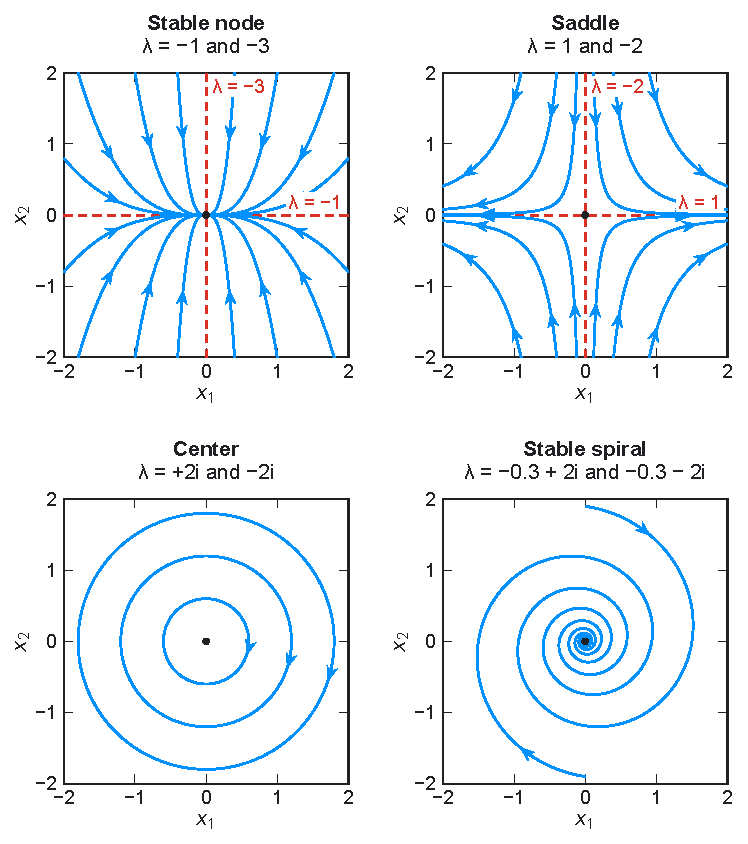
\includegraphics[width=\textwidth,height=0.50\paperheight,keepaspectratio,trim=0 204pt 0 0,clip]{assets/Fig-PhasePortraits.pdf}

  \vspace{0.3em}
  \raggedright
  A stable node draws every curve into the origin. A saddle brings curves in
  along the eigenvector of its negative eigenvalue and sends them out along
  the other.
  \lecturesource{Phase Portraits: the definition and the top row of the four-panel figure.
    Figure: ../figs/Fig-PhasePortraits/Fig-PhasePortraits.pdf (light TikZ build), top row.}
\end{frame}

\begin{frame}{Phase Portraits: Complex Eigenvalues}
  A complex pair of eigenvalues makes the solution curves turn around the
  steady state.

  \vspace{0.4em}
  \centering
  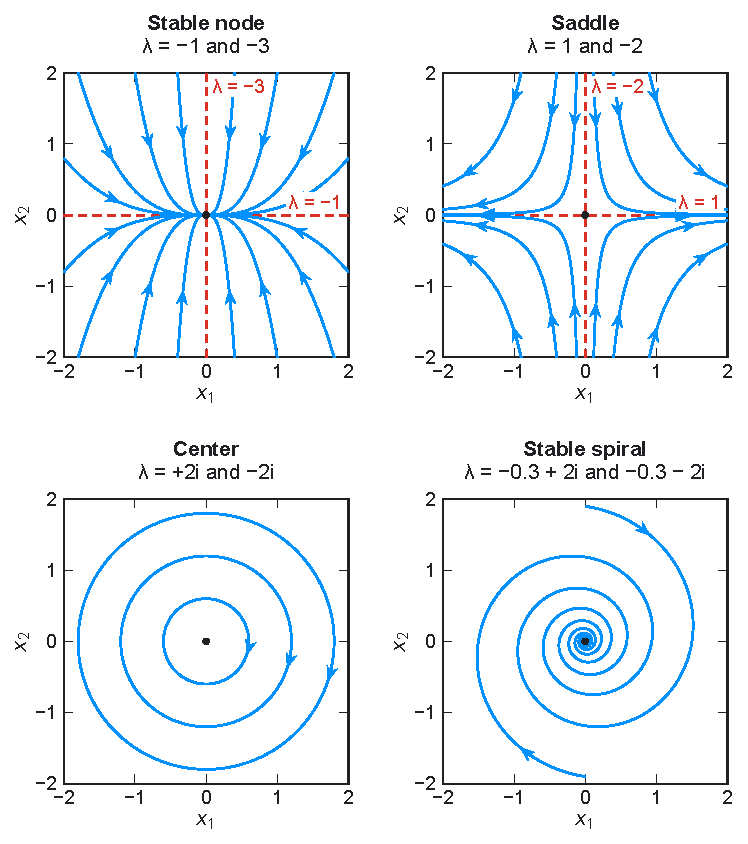
\includegraphics[width=\textwidth,height=0.50\paperheight,keepaspectratio,trim=0 0 0 201pt,clip]{assets/Fig-PhasePortraits.pdf}

  \vspace{0.3em}
  \raggedright
  A purely imaginary pair gives closed orbits, a center. A negative real part
  makes the curves spiral into the steady state.
  \lecturesource{Phase Portraits: the bottom row of the four-panel figure. Stability box: a purely imaginary pair gives an oscillation.
    Figure: ../figs/Fig-PhasePortraits/Fig-PhasePortraits.pdf (light TikZ build), bottom row.}
\end{frame}

\begin{frame}{The Forced Solution}
  Now suppose the input is not zero. We multiply the model by
  $e^{-\mathbf{A}t}$, which commutes with $\mathbf{A}$, and integrate:
  \begin{align*}
    \frac{d}{dt}\left(e^{-\mathbf{A}t}\mathbf{x}(t)\right) &= e^{-\mathbf{A}t}\mathbf{B}\mathbf{u}(t)
      && \text{product rule, in reverse}\\
    e^{-\mathbf{A}t}\mathbf{x}(t)-\mathbf{x}_{0} &= \int_{0}^{t}e^{-\mathbf{A}s}\mathbf{B}\mathbf{u}(s)\,ds
      && \text{integrate from } 0 \text{ to } t\\
    \mathbf{x}(t) &= e^{\mathbf{A}t}\mathbf{x}_{0}+\int_{0}^{t}e^{\mathbf{A}(t-s)}\mathbf{B}\mathbf{u}(s)\,ds
      && \text{multiply on the left by } e^{\mathbf{A}t}
  \end{align*}

  \vspace{0.2em}
  \begin{itemize}\setlength{\itemsep}{0.4em}
    \item The first term is the open-loop solution.
    \item The integral adds the effect of the input at every earlier time $s$,
      carried forward by the open-loop model over the remaining time $t-s$.
      For a general input, this integral has no closed form.
  \end{itemize}
  \lecturesource{The Forced Solution and Discretization: the derivation, condensed to three steps, and the paragraph after it.}
\end{frame}

\begin{frame}{The Trapezoid Rule}
  A \hilite{discretization} advances the state from one time to the next on a
  grid of times $t_{k}=k\Delta t$, with a step $\Delta t>0$. We derive two,
  and both hold the input constant at $\mathbf{u}_{k}\in\mathbb{R}^{d}$ over
  each step.

  \vspace{0.3em}
  The \hilite{trapezoid rule} approximates the integral of a function $g$
  over one step by the step times the average of its two end values:
  \[
    \int_{t_{k-1}}^{t_{k}}g(s)\,ds\approx\frac{\Delta t}{2}\left(g(t_{k-1})+g(t_{k})\right)
  \]
  We integrate the model over one step, and apply this rule to the state term:
  \[
    \left(\mathbf{I}-\tfrac{\Delta t}{2}\mathbf{A}\right)\mathbf{x}_{k}=\left(\mathbf{I}+\tfrac{\Delta t}{2}\mathbf{A}\right)\mathbf{x}_{k-1}+\Delta t\,\mathbf{B}\mathbf{u}_{k}
  \]
  where $\mathbf{x}_{k}$ approximates the state $\mathbf{x}(t_{k})$.
  \lecturesource{The Forced Solution and Discretization: the definition of a discretization. The Bilinear Discretization: the trapezoid rule and the derivation through the factored step.}
\end{frame}

\begin{frame}{The Bilinear Discretization}
  Multiplying through by the inverse of $\mathbf{I}-\tfrac{\Delta t}{2}\mathbf{A}$
  gives the discrete matrices $\bar{\mathbf{A}}\in\mathbb{R}^{n\times n}$ and
  $\bar{\mathbf{B}}\in\mathbb{R}^{n\times d}$:
  \[
    \boxed{\bar{\mathbf{A}}=\left(\mathbf{I}-\tfrac{\Delta t}{2}\mathbf{A}\right)^{-1}\left(\mathbf{I}+\tfrac{\Delta t}{2}\mathbf{A}\right),\qquad
    \bar{\mathbf{B}}=\left(\mathbf{I}-\tfrac{\Delta t}{2}\mathbf{A}\right)^{-1}\Delta t\,\mathbf{B}}
  \]
  The state follows the recursion, starting from $\mathbf{x}_{0}$:
  \[
    \mathbf{x}_{k}=\bar{\mathbf{A}}\mathbf{x}_{k-1}+\bar{\mathbf{B}}\mathbf{u}_{k},\qquad k=1,2,\dots
  \]

  \vspace{0.3em}
  The inverse exists when no eigenvalue of $\mathbf{A}$ equals $2/\Delta t$.
  Every stable model meets this condition.
  \lecturesource{The Bilinear Discretization: the last step of the derivation, the condition on the inverse, and the Bilinear discretization box.}
\end{frame}

\begin{frame}{The Bilinear Recursion Keeps Stability}
  Each eigenvector $\mathbf{v}$ of $\mathbf{A}$ is also an eigenvector of
  $\bar{\mathbf{A}}$, but its eigenvalue changes from $\lambda$ to
  $\bar{\lambda}$:
  \[
    \bar{\lambda}=\frac{1+\Delta t\,\lambda/2}{1-\Delta t\,\lambda/2},\qquad
    |\bar{\lambda}|<1\iff\mathrm{Re}(\lambda)<0
  \]
  \vspace{-0.2em}
  \begin{itemize}\setlength{\itemsep}{0.5em}
    \item Each mode of the recursion changes by the factor $\bar{\lambda}$ in
      each step, and it decays when $|\bar{\lambda}|<1$. A stable model gives a
      stable recursion, for any step $\Delta t$.
    \item The trapezoid rule makes the recursion second-order accurate: its
      error over a fixed time scales with $\Delta t^{2}$. Halving the step cuts
      the error by about a factor of four.
  \end{itemize}
  \slidenote{Derivation:}{\href{\bilinearlink}{Stability of the bilinear discretization}}
  \lecturesource{The Bilinear Discretization: the stability statement in the box and the accuracy paragraph. Examples section: the companion derivation.}
\end{frame}

\begin{frame}{The Zero-Order Hold}
  When the input is constant over each step, the forced solution gives the
  state at the end of each step exactly. Over one step, from $t_{k-1}$ to
  $t_{k}$:
  \begin{align*}
    \mathbf{x}(t_{k}) &= e^{\mathbf{A}\Delta t}\mathbf{x}(t_{k-1})+\int_{t_{k-1}}^{t_{k}}e^{\mathbf{A}(t_{k}-s)}\mathbf{B}\mathbf{u}(s)\,ds
      && \text{forced solution over one step}\\
    &= e^{\mathbf{A}\Delta t}\mathbf{x}(t_{k-1})+\left(\int_{0}^{\Delta t}e^{\mathbf{A}\sigma}\,d\sigma\right)\mathbf{B}\mathbf{u}_{k}
      && \mathbf{u}(s)=\mathbf{u}_{k}\text{, and } \sigma=t_{k}-s\\
    \mathbf{x}_{k} &= e^{\mathbf{A}\Delta t}\mathbf{x}_{k-1}+\mathbf{A}^{-1}\left(e^{\mathbf{A}\Delta t}-\mathbf{I}\right)\mathbf{B}\mathbf{u}_{k}
      && \text{antiderivative } \mathbf{A}^{-1}e^{\mathbf{A}\sigma}
  \end{align*}

  \vspace{0.2em}
  \begin{itemize}\setlength{\itemsep}{0.4em}
    \item No step is an approximation: $\mathbf{x}_{k}$ equals the state
      $\mathbf{x}(t_{k})$ at every grid time, for any step $\Delta t$.
    \item The \hilite{zero-order hold} is named for the constant input, a
      polynomial of order zero in time.
  \end{itemize}
  \lecturesource{The Zero-Order Hold Discretization: the opening paragraph and the two derivations, condensed to three steps, and the exactness statement.}
\end{frame}

\begin{frame}{The Zero-Order Hold Keeps Stability}
  The discrete matrices $\bar{\mathbf{A}}\in\mathbb{R}^{n\times n}$ and
  $\bar{\mathbf{B}}\in\mathbb{R}^{n\times d}$ give the same recursion,
  $\mathbf{x}_{k}=\bar{\mathbf{A}}\mathbf{x}_{k-1}+\bar{\mathbf{B}}\mathbf{u}_{k}$:
  \[
    \boxed{\bar{\mathbf{A}}=e^{\mathbf{A}\Delta t},\qquad
    \bar{\mathbf{B}}=\mathbf{A}^{-1}\left(e^{\mathbf{A}\Delta t}-\mathbf{I}\right)\mathbf{B}}
  \]
  Each eigenvalue $\lambda$ of $\mathbf{A}$ becomes $\bar{\lambda}$, with the
  same eigenvector:
  \[
    \bar{\lambda}=e^{\lambda\Delta t},\qquad
    |\bar{\lambda}|=e^{\mathrm{Re}(\lambda)\Delta t}<1\iff\mathrm{Re}(\lambda)<0
  \]
  \vspace{-0.2em}
  \begin{itemize}\setlength{\itemsep}{0.4em}
    \item The inverse of $\mathbf{A}$ exists when no eigenvalue is zero. A
      stable model gives a stable recursion, for any step $\Delta t$.
    \item The zero-order hold needs the matrix exponential. The bilinear
      discretization needs only the inverse of
      $\mathbf{I}-\tfrac{\Delta t}{2}\mathbf{A}$.
  \end{itemize}
  \lecturesource{The Zero-Order Hold Discretization: the condition on the inverse, the Zero-order hold discretization box, and the closing paragraph.}
\end{frame}

\begin{frame}{Linearization}
  Most models of real systems are nonlinear,
  $\dot{\mathbf{x}}=\mathbf{f}(\mathbf{x},\mathbf{u})$, where
  $\dot{x}_{i}=f_{i}(\mathbf{x},\mathbf{u})$ is the rate of change of state $i$,
  for $i=1,\dots,n$.

  \vspace{0.4em}
  \begin{itemize}\setlength{\itemsep}{0.4em}
    \item An \hilite{operating point} is any chosen state
      $\mathbf{x}_{\op}\in\mathbb{R}^{n}$ and input
      $\mathbf{u}_{\op}\in\mathbb{R}^{d}$.
    \item Near this point, we write the deviations
      $\Delta\mathbf{x}=\mathbf{x}-\mathbf{x}_{\op}$ and
      $\Delta\mathbf{u}=\mathbf{u}-\mathbf{u}_{\op}$. Because
      $\mathbf{x}_{\op}$ is constant, $\dot{\mathbf{x}}$ is also the rate of change
      of $\Delta\mathbf{x}$.
  \end{itemize}

  \vspace{0.3em}
  A first-order Taylor expansion of $\mathbf{f}$ about the operating point
  gives:
  \[
    \dot{\mathbf{x}}=\mathbf{f}(\mathbf{x}_{\op}+\Delta\mathbf{x},\,\mathbf{u}_{\op}+\Delta\mathbf{u})
    \approx\mathbf{f}(\mathbf{x}_{\op},\mathbf{u}_{\op})+\mathbf{A}\,\Delta\mathbf{x}+\mathbf{B}\,\Delta\mathbf{u}
  \]
  \lecturesource{Linearization: the nonlinear model, the operating point, the deviations, and the Taylor expansion.}
\end{frame}

\begin{frame}{Linearization about an Operating Point}
  Near the operating point, the deviations follow the model:
  \[
    \boxed{\dot{\mathbf{x}}\approx\mathbf{A}\,\Delta\mathbf{x}+\mathbf{B}\,\Delta\mathbf{u}+\mathbf{f}_{\op}}\qquad
    a_{ij}=\left.\frac{\partial f_{i}}{\partial x_{j}}\right|_{\op},\quad
    b_{ij}=\left.\frac{\partial f_{i}}{\partial u_{j}}\right|_{\op},\quad
    \mathbf{f}_{\op}=\mathbf{f}(\mathbf{x}_{\op},\mathbf{u}_{\op})
  \]
  \vspace{-0.2em}
  \begin{itemize}\setlength{\itemsep}{0.45em}
    \item $\mathbf{A}\in\mathbb{R}^{n\times n}$ is the \hilite{Jacobian} of
      $\mathbf{f}$ with respect to the state, and
      $\mathbf{B}\in\mathbb{R}^{n\times d}$ is the Jacobian with respect to the
      input, both evaluated at the operating point.
    \item The constant $\mathbf{f}_{\op}\in\mathbb{R}^{n}$ acts like an input
      that never changes. With the input $(\Delta\mathbf{u},1)$ and the input
      matrix $[\,\mathbf{B}\;\;\mathbf{f}_{\op}\,]$, the deviations follow the
      forced model, and both discretizations apply unchanged.
    \item The linear model is accurate only near the operating point. When
      $\mathbf{f}_{\op}\neq\mathbf{0}$, the state drifts, which can carry it
      away from the point.
  \end{itemize}
  \lecturesource{Linearization: the Linearization about an operating point box and the paragraph after it.}
\end{frame}

\begin{frame}{Linearization about a Steady State}
  A \hilite{steady state} $(\mathbf{x}^{\star},\mathbf{u}^{\star})$ of the
  nonlinear model satisfies $\mathbf{f}(\mathbf{x}^{\star},\mathbf{u}^{\star})=\mathbf{0}$.
  Steady states are the usual operating points, because the constant term
  vanishes there:
  \[
    \dot{\mathbf{x}}\approx\mathbf{A}\,\Delta\mathbf{x}+\mathbf{B}\,\Delta\mathbf{u}
  \]
  With the input held at $\mathbf{u}^{\star}$, the eigenvalues of $\mathbf{A}$
  decide whether small deviations decay or grow:
  \begin{itemize}\setlength{\itemsep}{0.45em}
    \item Every eigenvalue has a negative real part: small deviations decay,
      and the steady state is \hilite{stable}.
    \item One eigenvalue has a positive real part: a small deviation grows, and
      the steady state is \hilite{unstable}.
    \item An eigenvalue with zero real part leaves the question open.
  \end{itemize}
  \lecturesource{Linearization about a Steady State: the definition, the linear model, and the three cases.}
\end{frame}

\begin{frame}{Example: Linearizing a Gene Circuit}
  In this example, a settings cell picks one of three gene circuits and a
  pulse of the \hilite{inducer}, a small molecule that we add to the cells.
  Every task runs on the chosen circuit:

  \vspace{0.2em}
  \begin{enumerate}\setlength{\itemsep}{0.3em}
    \item Build the model from its config file, and solve the balances with
      an ODE solver.
    \item Find the steady state with the solver, and read the eigenvalues of
      the Jacobian there.
    \item Linearize the model about the steady state, solve it with the
      bilinear or the zero-order hold discretization, and compare it with the
      nonlinear model for the pulse.
  \end{enumerate}

  \vspace{0.2em}
  Change the settings or a config file, and rerun to see where the linear
  model holds and where it fails.
  \slidenote{Example:}{\href{\examplelink}{Linearize a gene circuit}}
  \lecturesource{Examples section: the example box. Companion example: the introduction, Tasks 1--3, Things to Try, and the key takeaways.}
\end{frame}

\begin{frame}{Summary}
  We solved linear state space models with and without an input, and
  linearized a nonlinear model about an operating point.

  \vspace{0.5em}
  {\large\textbf{\ink{Key takeaways}}}
  \vspace{0.3em}
  \begin{itemize}\setlength{\itemsep}{0.6em}
    \item \textbf{\ink{Eigenvalues decide stability.}} The model is stable when
      every eigenvalue has a negative real part.
    \item \textbf{\ink{Two discretizations of the forced model.}} Both keep the
      model's stability for any step. With the input held constant over each
      step, the zero-order hold gives the exact state at every grid time.
    \item \textbf{\ink{Linearization gives a local linear model.}} At a steady
      state, with the input held fixed, small deviations decay when every
      eigenvalue has a negative real part.
  \end{itemize}

  \vspace{0.5em}
  Together, these ideas predict how a nonlinear model responds to small changes
  in its state and input near an operating point.
  \lecturesource{Summary: three key takeaways and the closing paragraph.}
\end{frame}

\end{document}
